\chapter{GUI vodič}
\section{Prvi zagon}
Zaženemo skripto GUI.py, odprlo se nam bo okno, s pomočjo katerega se upravlja merilni sistem. Ob prvem zagonu se pomaknemo na zavihek \textit{Nastavitve} (slika \ref{fig:nastavitve}), kjer moramo izpolniti vsa polja. Pod Hostname, vpišemo hostname, ki smo ga določili v RPi (slika \ref{fig:pi_nast}). Če nismo spreminjali imena in gesla, sta ostala privzeta, in sicer ime: pi, geslo: raspberrypi. Na koncu vpišemo še pot do datoteke RPi\_MSLK.py.

Izpolnimo še kanala za krmiljenje zrcal. Pod \textit{Izhodni kanal 1} se vpiše kanal,  ki bo nadzoroval \textit{x} smer (\textit{x} je v smeri daljše stranice slike). Pod \textit{Izhodni kanal 2} pa kanal, ki nadzoruje \textit{y} smer.

Če imen kanalov ne poznamo, jih lahko pogledamo s pomočjo NiMAX, kjer se navigiramo do priklopljene kartice (slika \ref{fig:nimax}). Odčitamo ime in mu dodamo "/ao",ter številko želenega kanala. V našem primeru je tako ime prvega kanala za x smer: cDAQ10Mod1/ao0.
\begin{figure}[H]
    \centering
    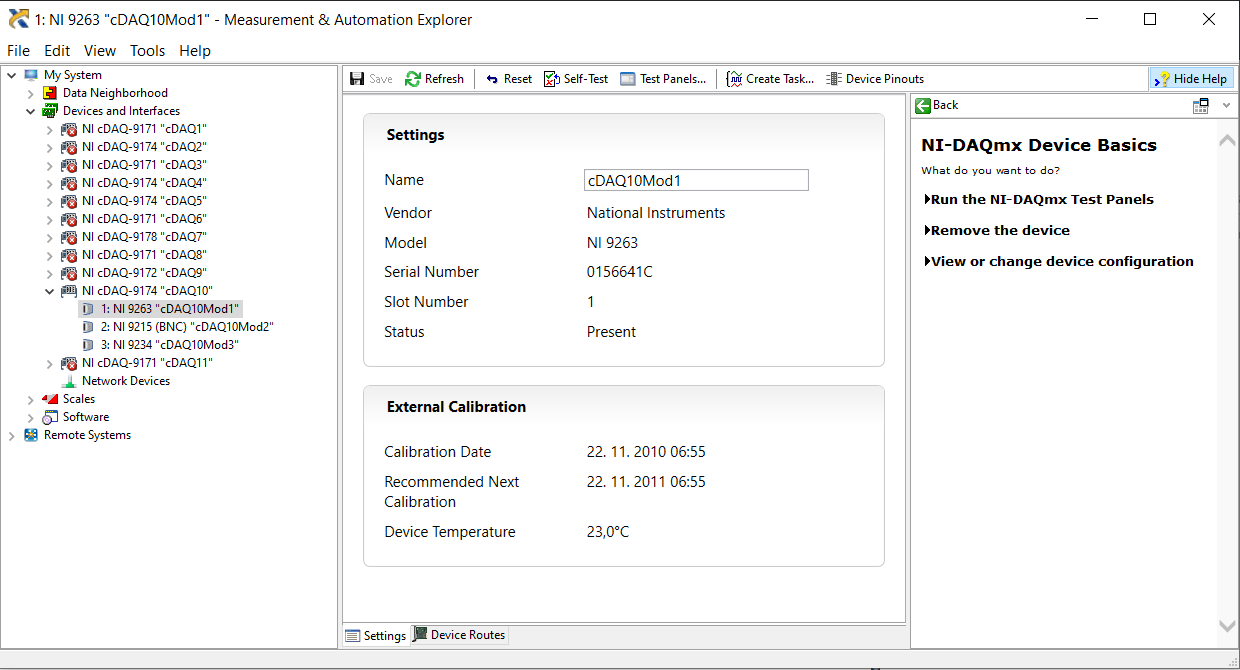
\includegraphics[width=\linewidth]{slike/nimax.png}
    \caption{Iskanje imena kanal s pomočjo NiMAX.}
    \label{fig:nimax}
\end{figure}

\section{Povezovanje na RPi}
Pred začetkom meritve se je potrebno povezati na RPi. To naredimo tako, da se pomaknemo na zavihek \textit{Kalibracija} (slika \ref{fig:tab1}), kjer se s pritiskom na zeleno tipko \textit{Vzpostavi povezavo}, vzpostavimo povezavo na RPi.  Če smo pravilo izpolnili vsa okna pod zavihkom \textit{Nastavitve}, se bo v nekaj sekundah vzpostavila povezava, prikaže se slika iz kamere, prav tako se zgodi kalibacija laserja.
\begin{figure}[H]
    \centering
    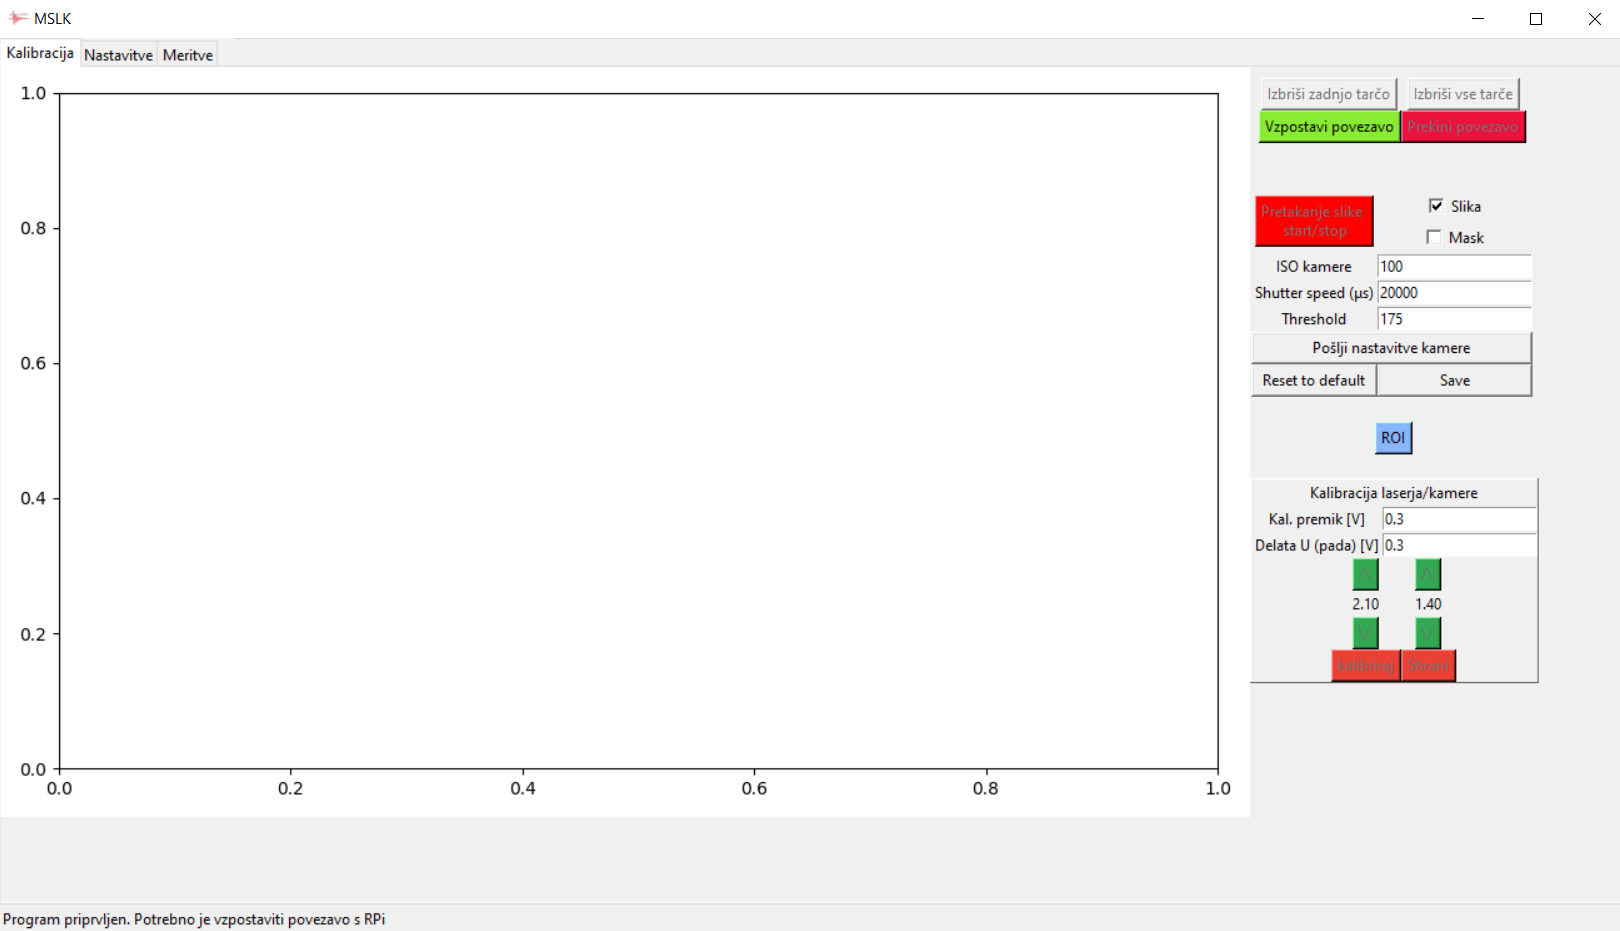
\includegraphics[width=.7\linewidth,trim = 200 145 0 0,clip]{slike/tabkalibracija.png}
    \caption{Zavihek Kalibracija.}
    \label{fig:tab1}
\end{figure}
V primeru, da je bil program predhodno nepravilno izklopljen, obstaja možnost, da se povezave prejšnje seje niso pravilno zaprle v tem primeru moramo narediti reboot sistemov.

\section{Kalibracija}
Ob povezavi se že avtomatsko zgodi kalibracija laserja, če je le ta slaba ali pa ni uspela, jo lahko ponovimo z ukazi pod \textit{Kalibracija laserja/kamere} (slika \ref{fig:tab1} na desni). Z zeleno obarvanimi tipkami spreminjamo vrednosti napetosti na posameznem zrcalu, za koliko se bo spremenila napetost na zrcalu (izpisana med zelenima tipkama) kontroliramo z vrednostjo, vnešeno v polje \textit{Delata U}. Ko laser postavimo na primerno mesto za kalibracijo, pritisnemo rdeči gumb \textit{kalibracija}, zgodi se kalibracijski premik za vrednost, podano pod \textit{Kal. premik}. Če želimo, da se bo takšna kalibracija zgodila ponovno, ob naslednji povezavi pritisnemo gumb \textit{Shrani}.

\section{Izbira ROI}
V primeru, da je v vidnem polju moteč dejavnik (npr. močan vir svetlobe), ki programu preprečuje, da bi zaznal žarek, lahko izberemo manjše območje interesa (ROI). To storimo s klikom na gumb ROI, nato pa kliknemo na ekran, da določimo meje območja. S tem smo omejili iskanje žarka le na območje, ki je označeno, ki ga obdaja oranžen okvir. Pri tem moramo paziti, da nam žarek ne zaide izven omenjenega območja, saj ga v tem primeru ne bo mogoče zaznati. Prav tako morajo vse tarče ležati znotraj ROI.


\section{Izbira tarč}
Ko imamo sliko, lahko tarče preprosto izbiramo tako, da kliknemo na željeno meso na sliki. Prikaže se zelen kvadratek ter oznaka tarče. V primeru, da smo se zmotili, lahko s pritiskom na gumb \textit{Izbriši zadnjo tarčo} izbrišemo tarčo, ki je bila zadnja dodana. Če želimo izbrisati vse tarče, kliknemo \textit{Izbriši vse tarče}.

\section{Nastavitve slike}
Če želimo spremljati trenutno sliko, pritisnemo na gumb \textit{Pretakanje slike, start/stop}. Iz RPi se bo začele pridobivati slike z nastavitvami kamere, ki so vpisana v polja \textit{ISO} (vrednosti od 100-800) in \textit{Shutter speed} (vrednosti do 6000000). Kamera bo prejela nove nastavitve po pritisku gumba \textit{Pošlji nastavitve kamere}. Program omogoča spremljane zajete slike ali pa slike, ki se uporablja za iskanje laserskega žarka (izbira \textit{Slika} ali \textit{Mask}).

\section{Nastavitve}

Pred začetkom meritev je v zavihku \textit{Nastavitve} potrebno nastaviti še ostale dele merilnega sistema. Pri vsakem sklopu nastavitev sta gumba \textit{Reset to default} in \textit{Save}, s katerima nadzorujemo shranjevanje sklopa nastavitev.
\subsection{Nastavitve RPi}
Te nastavitve je potrebno izpolniti že pred vzpostavljanjem povezave na RPi.


\begin{figure}[H]
    \centering
    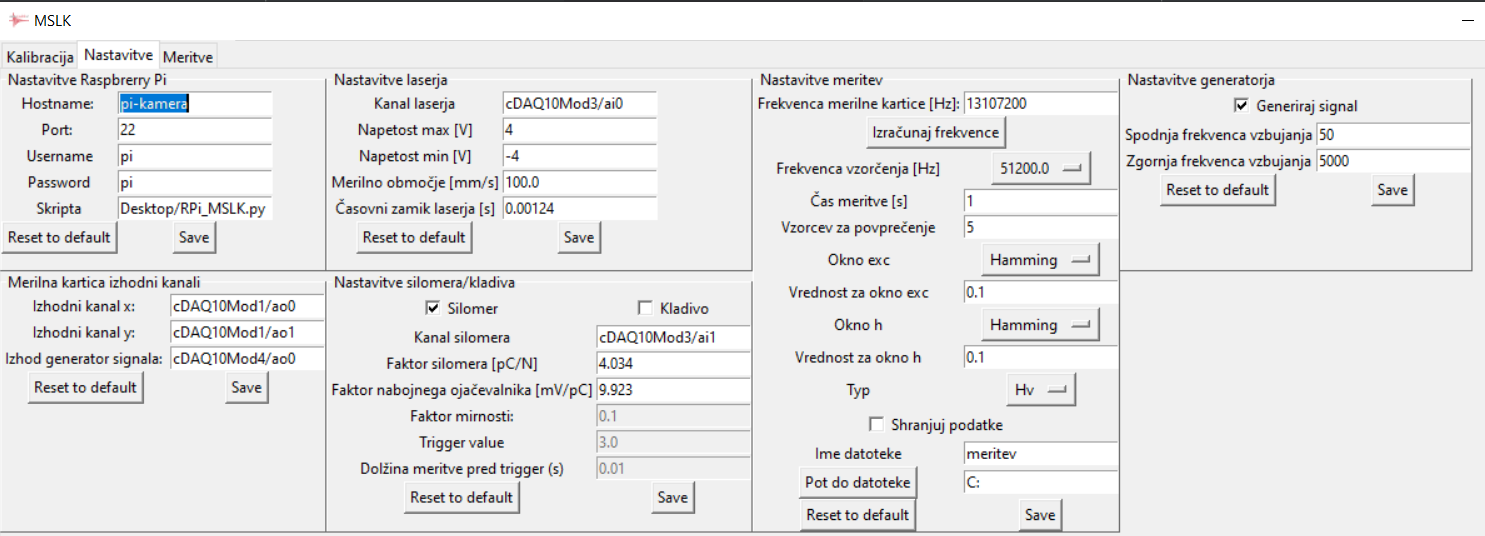
\includegraphics[width=.9\linewidth,trim=0 0 0 25,clip]{slike/zavihek_nastavitve.png}
    \caption{Nastavitve}
    \label{fig:nastavitve}
\end{figure}
\subsection{Nastavitve merilne kartice-izhodni kanali}
Potrebno je izbrati izhodne kanale za nadzor zrcal in generiranje vzbujevalnega signala. Paziti moramo, da so kanali za generiranje signala na drugi kartici kot kanali za krmiljenje zrcal.
\subsection{Nastavitve laserja}
Nastaviti je potrebno vhodni kanal laserja, napetost, pri kateri operira merilno območje, in časovni zamik.
\subsection{Nastavitve silomera/kladiva}
Prvo izberemo, ali bomo meritev izvajali s silomerom ali kladivom, glede na izbiro se nam omogoči spreminjanje vrednosti relevantnih polj. Ponovno določimo vhodni kanal (IEPE) ter faktorje ojačanja. V primeru meritev s kladivom določimo še faktor mirnosti. Ta predstavlja odstotek merilnega območja laserja, do katerega se mora umiriti objekt (max-min vrednost znotraj časa meritve), poredno je dovoljeno izvajanje meritev. Trigger value predstavlja vrednost, ki jo je potrebno preseči, da se začne meritev (samo pri kladivu).
\subsection{Nastavitve meritev}
Nastaviti moramo osnovno frekvenco merilne kartice, nato s klikom na gumb \textit{Izračunaj frekvence} osvežimo nabor možnih frekvenc vzorčenja.
Pod čas meritve določimo, koliko časa se bo izvajala posamična meritev mesta, z vzorcev za povprečenje pa določimo, koliko meritev se bo izvedlo na posameznem mestu. Določimo še okno za vzbujevalni signal (exc) in odziv (h) ter vrednosti oken (\href{https://github.com/openmodal/pyFRF/blob/master/pyFRF.py}{pyFRF}). Če želimo shranjevati podatke, moramo odkljukati okno shranjuj podatke ter določiti mesto in ime datoteke.
\subsection{Nastavitve generatorja}
Če želimo vzbujati s signalom, generiranim s pomočjo merilne kartice, moramo označiti \textit{generiraj signal}. Nastavljamo še lastnosti signala, s katerim želimo vzbujati naš objekt spodnjo in zgornjo mejo PSD. 


\newpage
\section{Meritev}
Za začetek meritev se pomaknemo na zavihek \textit{Meritve} (slika \ref{fig:tab3}).
\begin{figure}[H]
    \centering
    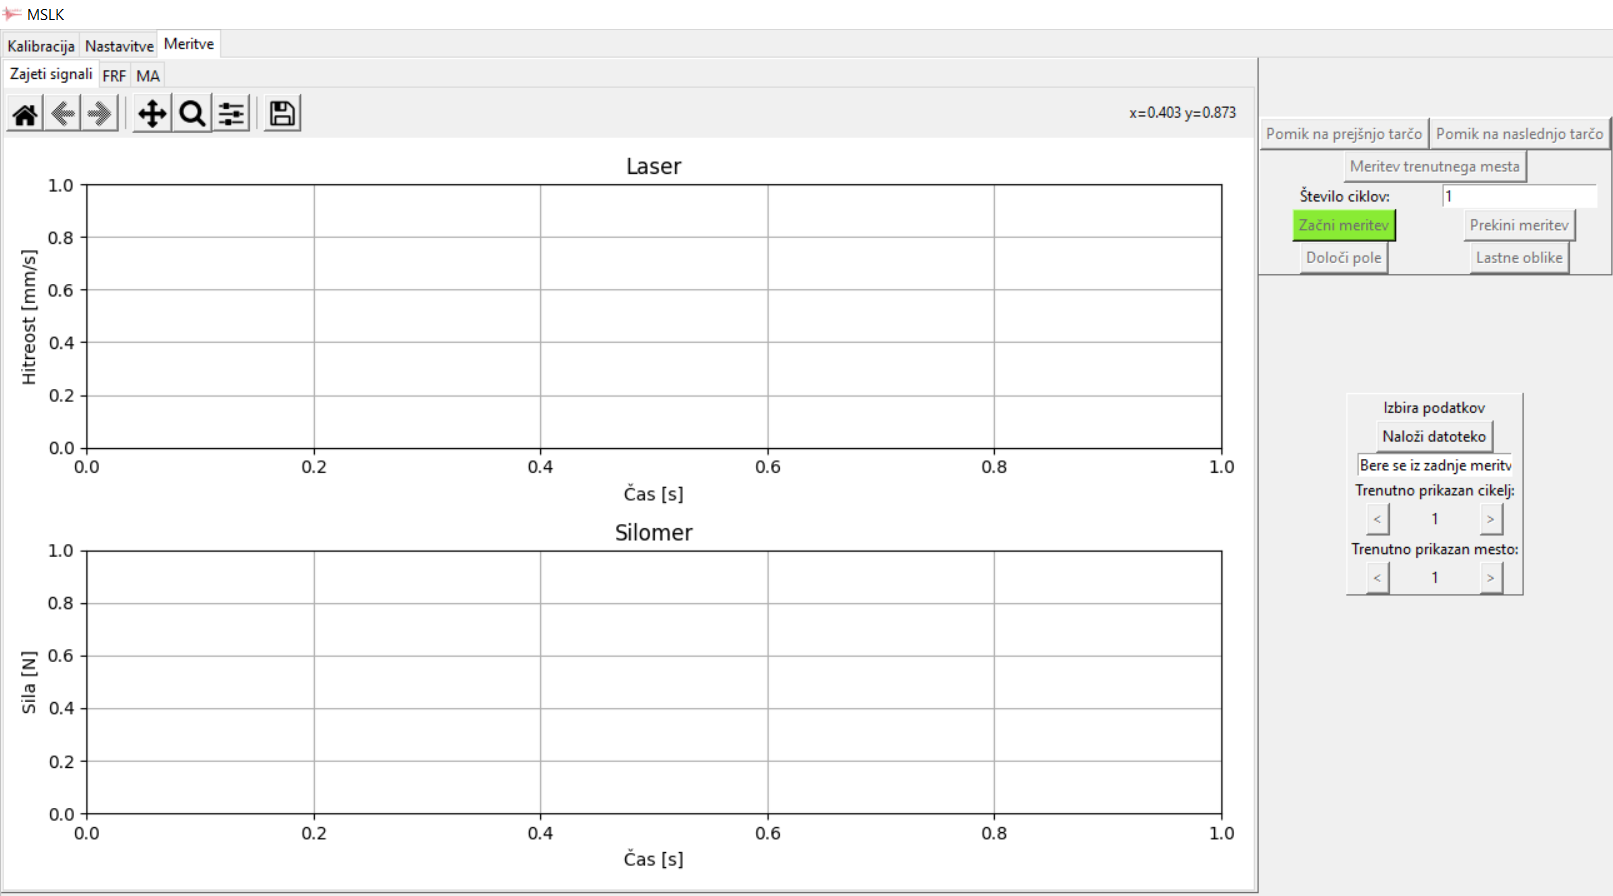
\includegraphics[width=0.9\linewidth]{slike/meritve.png}
    \caption{Zavihek meritve.}
    \label{fig:tab3}
\end{figure}
Če želimo izvesti meritev samo v določeni točki, se lahko na to točko pomaknemo z gumbi \textit{Pomik na prejšnjo tarčo} in \textit{Pomik na naslednjo tarčo}. Ko se laser nahaja na želeni poziciji, začnemo meritev z gumbom \textit{Meritev trenutnega mesta}.

Če želimo izvesti meritev na vseh označenih mestih, kliknemo gumb \textit{Začni meritev}. Laser se bo pomaknil na prvo mesto, izvedel meritev ter nato pomaknil naprej na naslednje mesto. Pomik in izvajanje meritev skozi vsa mesta (cikel) se izvede tolikokrat, koliko ciklov smo določili v polju \textit{Število ciklov}.

\subsection{Preko silomera}
V primeru, da merimo s pomočjo silomera (vzbujamo s ''stinger-jem''), samo zaženemo meritev, laser se bo premikal od tarče do tarče, dokler niso izvedene vse meritve.
\subsection{S kladivom}
Ko zaženemo meritev, se laser pomakne v prvo točko, ko se objekt dovolj umiri, (\textit{Nastavitve/faktor mirnosti}) zaslišimo zvok (dolg pisk, kratek pisk). To pomeni, da lahko udarimo s kladivom, če je bila meritev uspešna, se izriše FRF, v nasprotnem primeru zaslišimo zvok (kratek pisk, dolg pisk). Če je bila meritev uspešna, bo program počakal, da se merjenec ponovno umiri, predno se bo pomaknil na naslednje merilno mesto. Ponovno počakamo na zvok za začetek meritve.
\section{Določanje lastnih oblik}
Ko smo naredili meritev na vseh mestih, lahko izračunamo še lastne oblike. Prvo je potrebno določiti pole, kar naredimo s pritiskom na gumb \textit{Določi pole}. Odpre se nam novo okno, kje izberemo pole. Ko smo izbrali pole, lahko zapremo okno (v katerem smo izbirali pole) ter kliknemo gumb \textit{Plotaj lastne oblike}.
